\chapter{传感原理和敏感元件}
\label{chap:hw-sensors}

\noindent 本章对应《课后作业-CH4》的全部7题。各题沿着“被测量改变什么物理量，测量电路怎样读出，哪些条件限制结论”展开；所列应用均用于解释原题，不另设练习。

\section{第1题：应变片电阻变化与电流表的可读性}
\label{sec:hw-sensors-1}
\label{hw:4-1}
\begin{hwquestion}
电阻应变片的灵敏度 $S_g=2$，初始电阻 $R=120\,\Omega$，工作应变为 $1000\,\mu\varepsilon$。求 $\Delta R$。将应变片与原图中的 $1.5\,\mathrm V$ 电源、电流表串联，求：（1）无应变时电流；（2）有应变时电流；（3）电流指示值的相对变化量；（4）分析该变化能否从表中读出。
\end{hwquestion}

\subsection*{答案与解析}
按正应变表示拉伸，忽略电源内阻、电流表内阻及导线电阻，供电电压恒为 $U=1.5\,\mathrm V$。先换算应变：
\[
\varepsilon=1000\times10^{-6}=10^{-3},\qquad
\frac{\Delta R}{R}=S_g\varepsilon=0.002.
\]
因此
\[
\boxed{\Delta R=RS_g\varepsilon=0.24\,\Omega},\qquad
R'=R+\Delta R=120.24\,\Omega.
\]
电流表的两个读数为
\[
\boxed{I_0=\frac{1.5}{120}=12.5\,\mathrm{mA}},\qquad
\boxed{I=\frac{1.5}{120.24}\approx12.47505\,\mathrm{mA}}.
\]
由此得到电流的绝对变化与相对变化：
\begin{align*}
\Delta I&=I-I_0\approx-0.02495\,\mathrm{mA}=-24.95\,\mu\mathrm A,\\
\boxed{\frac{\Delta I}{I_0}}
&=\frac{R}{R+\Delta R}-1
=-\frac{\Delta R/R}{1+\Delta R/R}
=\boxed{-0.001996\approx-0.1996\%}.
\end{align*}
正应变使电阻增大，恒压供电下电流减小。若只作一阶近似，则 $\Delta I/I_0\approx-\Delta R/R=-0.2\%$；精确结果的分母不能省略。

\textbf{能否读出：}原题未给电流表的量程、最小分度或数字分辨力，也未给噪声和漂移，因而不能作唯一判断。要可靠区分两个读数，表计应能分辨约 $25\,\mu\mathrm A$ 的变化，且重复读数的噪声、供电变化和温漂须足够小。该变化仅约占初始读数的 $0.2\%$，普通粗分度毫安表通常难以清楚辨别；合适的精密表计则可能读出。若使用准确度按满量程给出的模拟表，还需结合所选量程评估读数可信程度。

\subsection*{本题知识点与公式}\label{kn:4-1}
\noindent\textbf{本题新增：}建立“构件变形 $\to$ 敏感栅应变 $\to$ 电阻变化 $\to$ 电流或桥压”的完整关系。本题先讲应变计本体，完整单臂、半桥和全桥接线在信号调理部分继续展开。

\subsubsection*{1. 应变、电阻与灵敏度系数从何而来}
轴向工程应变定义为 $\varepsilon=\Delta l/l_0$，其中 $l_0$ 是未变形长度，$\Delta l$ 是沿所选方向的长度增量。应变无量纲，通常拉伸为正、压缩为负；$1\,\mu\varepsilon=10^{-6}$。它与应力不同：应力单位为Pa，单轴、小变形、线弹性条件下才有 $\sigma_m=E\varepsilon$，其中 $E$ 是杨氏模量。

均匀导体电阻满足
\[
R=\rho\frac{l}{A_s},\qquad
\frac{\diff R}{R}=\frac{\diff\rho}{\rho}
+\frac{\diff l}{l}-\frac{\diff A_s}{A_s}.
\]
$\rho$ 为电阻率（$\Omega\,\mathrm m$），$A_s$ 为敏感栅截面积（$\mathrm m^2$）。式中三个来源分别是材料电阻率改变、长度改变及截面积改变，不能只保留长度项。若敏感栅近似承受单轴应变，泊松比 $\nu=-\varepsilon_{\perp}/\varepsilon$，两横向尺寸相对应变均为 $-\nu\varepsilon$，则一阶近似有
\[
\frac{\Delta A_s}{A_s}\approx-2\nu\varepsilon,
\quad
\frac{\Delta R}{R}\approx(1+2\nu)\varepsilon+\frac{\Delta\rho}{\rho}.
\]
于是应变片灵敏度系数为
\[
\boxed{S_g=\frac{\Delta R/R}{\varepsilon}
\approx1+2\nu+\frac{\Delta\rho/\rho}{\varepsilon}},
\qquad \Delta R\approx RS_g\varepsilon.
\]
这里以小变化比值代表局部导数；$S_g$ 无量纲，应采用制造商标定值或题给值。\textbf{金属应变片}中几何变化很重要，电阻率变化也可能贡献，常见 $S_g$ 约为2；\textbf{半导体应变片}的压阻效应使电阻率随应力明显改变，通常灵敏度更大，但温度影响、非线性与个体差异也更显著。故不能把所有材料的 $S_g$ 都固定成 $1+2\nu$。

\subsubsection*{2. 应变片测的是哪个方向的应变}
粘贴式应变片依靠基底和胶层把构件表面变形传到敏感栅，主要测量栅轴方向的平均应变。栅线需与所求应变方向一致，粘贴不良、胶层蠕变和局部应变梯度都会改变读数。若表面平面应变分量为 $\varepsilon_x,\varepsilon_y,\gamma_{xy}$，栅轴相对 $x$ 方向夹角为 $\theta$，则
\[
\varepsilon_\theta=\varepsilon_x\cos^2\theta+
\varepsilon_y\sin^2\theta+\gamma_{xy}\sin\theta\cos\theta.
\]
$\gamma_{xy}$ 是工程剪应变，等于张量剪应变的两倍；角度误差不一定只造成一个余弦系数。未知主应变方向时，可用多个方向的应变片组成应变花，再由各方向读数重建应变状态。原题默认给定的 $1000\,\mu\varepsilon$ 就是栅轴方向的有效应变。

\subsubsection*{3. 温度交叉影响与激励自热}
温度既能改变敏感栅电阻率，也会引起栅、基底和构件的热膨胀不匹配。把这些影响在工作点附近合并为有效温度系数 $\alpha_{\mathrm{eff}}$（$\mathrm K^{-1}$），可写
\[
\frac{\Delta R}{R}\approx S_g\varepsilon+
\alpha_{\mathrm{eff}}\Delta T,\qquad
\varepsilon_{\mathrm{app}}=\frac{\alpha_{\mathrm{eff}}\Delta T}{S_g}.
\]
第二项会被误读为表观应变；$\alpha_{\mathrm{eff}}$ 随材料和安装条件而定，并非单一材料电阻温度系数的通用替代。温度还会改变 $S_g$，因此零点补偿和灵敏度温度补偿是两个问题。可采用匹配材料的自温度补偿片、同温补偿片和合理桥路减轻影响，仍须按实际温度范围标定。

电阻上的激励功率为 $P_g=I_g^2R=U_g^2/R$。提高激励会增大可测信号，同时增加自热；温升又反过来引起电阻漂移。应检查应变片允许功率、栅面积和构件散热条件，不能只为提高输出无限增大供电。\footnote{应变、桥路与温度补偿的器件说明可参见\href{https://www.ni.com/en/shop/data-acquisition/sensor-fundamentals/measuring-strain-with-strain-gages.html}{NI：Measuring Strain with Strain Gages}。}

\subsubsection*{4. 从电阻变化到可辨读数}
若串联回路还有固定电阻 $R_s$，则
\[
I(\varepsilon)=\frac{U}{R(1+S_g\varepsilon)+R_s},\quad
I_0=\frac{U}{R+R_s},\quad
\frac{\Delta I}{I_0}=-\frac{RS_g\varepsilon}{R+R_s+RS_g\varepsilon}.
\]
在零应变附近，电流对应变的局部灵敏度为
\[
S_{I\varepsilon}=\left.\frac{\diff I}{\diff\varepsilon}\right|_0
=-\frac{URS_g}{(R+R_s)^2},\qquad
\Delta\varepsilon_{\min}\approx\frac{\Delta I_{\min}}{|S_{I\varepsilon}|}.
\]
$S_{I\varepsilon}$ 的单位为A/应变，$\Delta I_{\min}$ 是电流输出端可辨变化；折算成微应变时应乘 $10^6$。由此可见，表内阻和引线电阻不仅改变基值，也会降低相对应变的读出能力。原题还缺少 $\Delta I_{\min}$、噪声及漂移，因此不能仅由理论 $\Delta I$ 断言仪表一定可读。

平衡电桥用两个分压点相减，把未受力时的大基值抵消，使微小变化便于差分放大。等臂、单臂变化、输出近似开路时，有
\[
|U_o|\approx\frac{U_e}{4}\left|\frac{\Delta R}{R}\right|
=\frac{U_eS_g}{4}|\varepsilon|.
\]
它说明电桥为何适合本题的微小电阻变化；准确系数、符号及半桥、全桥增敏条件须由具体接线推导，不能只按应变片数量判断。
\nt{\textbf{易错点：}$1000\,\mu\varepsilon=0.001$，不是 $0.001\%$；相对电阻变化为 $+0.2\%$，电流相对变化约为 $-0.1996\%$。分辨力说明能否区分变化，准确度还涉及偏差等因素，两者不能混用。}

\needspace{11\baselineskip}
\section{第2题：电容、电感和电阻应变式测量电路的异同}
\label{hw:4-2}
\begin{hwquestion}
电容式、电感式、电阻应变式传感器的测量电路有何异同？举例说明。
\end{hwquestion}

\subsection*{答案与解析}
\textbf{共同点：}三者都可先把被测量转换为电参数变化，即 $\Delta C$、$\Delta L$ 或 $\Delta R$，再借助外部激励和转换电路得到可测电压、电流或频率。测量链通常包含激励、参数转换、放大、必要的解调及滤波；差动结构、电桥和比值读出均可用于抑制部分共同干扰。

\begin{center}
\small
\begin{tabularx}{\linewidth}{@{}p{1.6cm} X X@{}}
\toprule
类型 & 典型读出电路与例子 & 主要区别和误差来源 \\
\midrule
电阻应变式 & 直流或交流电阻桥。应变使 $\Delta R/R=S_g\varepsilon$，桥路把电阻比变化变成差分电压。 & 可直接用直流激励；须注意导线电阻、供电稳定性、自热和温度补偿。 \\
电容式 & 交流电桥、交流阻抗分压、充放电计时或振荡调频。变极距位移使 $C=\varepsilon_0\varepsilon_r A/d$ 改变。 & $Z_C=1/(\iu\omega_e C)$；电容量常较小，对寄生电容、漏电、屏蔽和前端输入阻抗敏感。 \\
电感式 & 交流电桥、阻抗分压、差动变压器或振荡调频。气隙变化引起 $L$ 改变；差动变压器读二次差动电压。 & 线圈一般含 $R_w+\iu\omega_e L$，需考虑绕组电阻、磁滞、漏磁、损耗及外磁场；相位信息常有意义。 \\
\bottomrule
\end{tabularx}
\end{center}

直流电阻桥在理想条件下的平衡关系只涉及电阻比例；交流桥的平衡关系涉及\textbf{复阻抗比例}，通常须同时满足幅值与相位条件。对电容或电感施加恒定直流并等待暂态消失，不能仅由理想元件的稳态电压、电流读出其参数；因此常用交流或充放电等时变过程测量。

\subsection*{本题知识点与公式}\label{kn:4-2}
\noindent\textbf{已学前置：}\hyperref[kn:4-1]{第1题}已建立电阻应变转换与外部激励读出。本题新增电容、自感、互感的结构关系，以及三类参数共有的交流桥、时间和频率读出。频率响应的幅相概念见\hyperref[kn:3-1]{测试系统第1题知识点}。

\subsubsection*{1. 电容式：面积、极距和介质三种结构}
忽略边缘效应的平行板电容为
\[
C=\frac{\varepsilon_0\varepsilon_rA}{d},\qquad
\frac{\diff C}{C}=\frac{\diff\varepsilon_r}{\varepsilon_r}
+\frac{\diff A}{A}-\frac{\diff d}{d}.
\]
$C$ 的单位是F，$\varepsilon_0$ 为真空介电常数（F/m），$\varepsilon_r$ 为无量纲相对介电常数，$A$ 为有效重叠面积，$d$ 为极距。\textbf{变极距型}用膜片或动极板改变 $d$，局部灵敏度 $\diff C/\diff d=-\varepsilon_0\varepsilon_rA/d^2$；极距越小越灵敏，但允许行程、机械平行度、击穿和碰撞风险也更严格。若 $x>0$ 表示极距缩小，
\[
C(x)=\frac{C_0}{1-x/d_0},\qquad
\frac{\Delta C}{C_0}=\frac{x/d_0}{1-x/d_0}\approx\frac{x}{d_0}
\quad(|x|\ll d_0).
\]
\textbf{变面积型}保持极距不变，矩形极板重叠面积 $A=bx$ 时，$C=\varepsilon_0\varepsilon_r bx/d$，理想灵敏度为常数 $\varepsilon_0\varepsilon_r b/d$，适合较大位移或角位移。\textbf{变介质型}使介电常数或介质占据比例改变；例如介质沿极板长度方向插入、不同区域相当于并联时，
\[
C(x)=\frac{\varepsilon_0 b}{d}
\bigl[\varepsilon_r x+(l-x)\bigr].
\]
这里 $l$ 为极板总长，外部区域取空气；若介质沿电场方向分层，应按串联电容处理，不能直接沿用此式。液位、厚度和湿度测量都需明确几何与介质分布。

\textbf{差动结构的推导：}两侧间隙为 $d_0-x$、$d_0+x$，令 $r=x/d_0$，则
\[
C_1=\frac{C_0}{1-r},\quad C_2=\frac{C_0}{1+r},\quad
\frac{C_1-C_2}{C_0}=\frac{2r}{1-r^2},\quad
\boxed{\frac{C_1-C_2}{C_1+C_2}=r}.
\]
差值在零点附近灵敏度加倍并消除偶次项；\textbf{差值本身仍非严格线性，理想差和比才严格线性}。极板不平行、寄生电容和边缘效应会破坏理想关系。电容量小时，引线电容可能与信号同量级，需短引线、屏蔽、保护环或就近前置读出。

\subsubsection*{2. 自感、互感与涡流并非同一种转换链}
磁路近似中，磁动势 $NI=\mathcal R_m\Phi$，磁链 $\lambda_m=N\Phi$，由 $L=\lambda_m/I$ 得
\[
\boxed{L\approx\frac{N^2}{\mathcal R_m}},\qquad
\mathcal R_m=\sum_i\frac{l_i}{\mu_iA_i}.
\]
$N$ 为线圈匝数，$I$ 为电流（A），$\Phi$ 为磁通（Wb），$\lambda_m=N\Phi$ 为磁链；$L$ 的单位为H，$\mathcal R_m$ 为磁阻（A/Wb），$l_i,A_i$ 为第 $i$ 段磁路长度与截面积，$\mu_i$ 为磁导率（H/m）。若铁芯磁阻可忽略，总气隙长度为 $g$，则 $L\approx N^2\mu_0A/g$，有 $\diff L/\diff g=-L/g$。可变气隙式用位移改变磁阻；公式要求磁通近似均匀、漏磁和边缘效应较小且磁芯未饱和。

互感型通过一次线圈激励在二次线圈产生感应电压。差动变压器（LVDT）含两个反向串联的二次线圈，铁芯居中时互感近似相等。用一次电流相量 $I_p$ 表示，
\[
U_d=\iu\omega_e(M_1-M_2)I_p.
\]
在中心附近设 $M_1=M_0+k_Mx$、$M_2=M_0-k_Mx$，则 $U_d\approx\iu2\omega_e k_MI_px$。所以幅值反映位移大小，跨过零点时符号改变，等效载波相位翻转 $180^\circ$。实际若采用电压激励，一次电流还受一次阻抗影响；常用标定后的 $U_d\approx K_xxU_e$ 描述，不能把 $K_x$ 当成与激励频率无关的常数。\footnote{LVDT的耦合与同步解调见\href{https://www.analog.com/en/resources/reference-designs/circuits-from-the-lab/cn0371.html}{Analog Devices：CN0371}。}

涡流式则由交流磁场在导体中激发涡流，反作用使线圈的\textbf{等效电阻和电感同时变化}，读出量是 $Z=R_{\mathrm{eq}}+\iu\omega_eL_{\mathrm{eq}}$。间距、导电率、磁导率和缺陷都可能改变 $Z$；材料与检测深度问题在\hyperref[kn:4-5]{第5题}详细展开。

\subsubsection*{3. 从参数到时间、频率或桥压}
三种基本阻抗为 $Z_R=R$、$Z_C=1/(\iu\omega_e C)$、$Z_L=\iu\omega_e L$；实际电容有漏电和介质损耗，线圈有绕组电阻。\textbf{RC计时}利用 $U_C(t)=U_e(1-e^{-t/RC})$：达到固定阈值 $U_{\mathrm{th}}$ 所需时间为
\[
t_{\mathrm{th}}=-RC\ln\!\left(1-\frac{U_{\mathrm{th}}}{U_e}\right).
\]
在 $R$ 和阈值比固定时，$t_{\mathrm{th}}\propto C$；它可读静态电容，并不需要被测对象持续运动。\textbf{LC调频}利用 $f_r=(2\pi\sqrt{LC})^{-1}$，对数微分得到
\[
\frac{\Delta f_r}{f_r}\approx-\frac12
\left(\frac{\Delta L}{L}+\frac{\Delta C}{C}\right).
\]
固定一项即可读另一项；寄生参数、损耗和振荡器稳定性也会影响频率。

\textbf{交流桥的一般平衡：}规定左支路上、下臂为 $Z_1,Z_2$，右支路上、下臂为 $Z_3,Z_4$，桥源加在上下端，输出取左中点减右中点。输出开路时，
\[
U_o=U_e\left(\frac{Z_2}{Z_1+Z_2}-\frac{Z_4}{Z_3+Z_4}\right),\qquad
\boxed{Z_1Z_4=Z_2Z_3\ \Longleftrightarrow\ U_o=0}.
\]
交流平衡不仅要求阻抗模的比例匹配，还要求相角差匹配；纯电阻桥是其特例。若信号为 $u_s=A(x)\cos(\omega_et+\phi)$，与同频参考 $\cos\omega_et$ 相乘再低通，保留 $A(x)\cos\phi/2$。相敏读出因此能保留载波正反相对应的位移符号；单纯取绝对幅值会丢失方向。实际需先校准载波相差，且解调低通应通过被测变化、抑制高频乘积项。
\nt{\textbf{易错点：}“需要交流激励”不等于“只能测动态量”。静态位移也可使电容或电感保持在新值，再由持续交流激励读出。被测量变化频率与激励载波频率应分别标明。}

\needspace{11\baselineskip}
\section{第3题：光电传感器的类型、特点与被测量}
\label{hw:4-3}
\begin{hwquestion}
光电传感器包含哪几种类型？各有何特点？用光电式传感器可以测量哪些物理量？
\end{hwquestion}

\subsection*{答案与解析}
若按\textbf{光电转换的物理效应}分类，可分为以下三类；后两类均属于内光电效应。
\begin{enumerate}
\item \textbf{外光电效应型：}光子使电子逸出材料表面，由阳极收集形成电流。典型元件为光电管、光电倍增管；倍增管通过二次电子发射获得较高增益，适合弱光检测，但通常需高压供电，并应注意强光、背景光和噪声。
\item \textbf{光导效应型：}光照在材料内部产生或释放载流子，改变电导率。典型元件为光敏电阻，通常光照增强时电阻降低，需要外加电源读出；结构简单，但响应速度、线性、暗电阻与温度影响取决于材料。
\item \textbf{光生伏特效应型：}光生电子、空穴被结区内建电场分离，形成光电流或光电压。典型元件为光电池和以光伏模式工作的光电二极管；可在零外加偏压下检测光，但输出仍需合适电路读出。
\end{enumerate}
光电二极管也可反向偏置运行以改善速度等性能，此时常称光导模式；不能因此把它的工作过程等同于光敏电阻的电阻变化。

若按\textbf{光路布置}分类，又可说对射式、反射式、遮光式等；若按信息编码方式分类，可说模拟光强测量、脉冲计数、成像等。它们与上述物理效应分类处于不同层面，可相互组合。

\begin{center}
\small
\begin{tabularx}{\linewidth}{@{}p{2.8cm} X@{}}
\toprule
可测物理量 & 被测量到光电信号的转换关系 \\
\midrule
光强、光功率、照度 & 直接检测入射光；须匹配光谱响应并进行相应标定。 \\
位移、尺寸、振动 & 位移改变遮挡面积、反射光耦合或光斑位置，产生连续电信号。 \\
转速、角位移、计数 & 光栅或码盘周期遮光，把运动变为脉冲频率、相位或脉冲数。 \\
温度 & 目标热辐射的光强或光谱随温度变化，结合辐射模型与发射率求温度。 \\
浓度、液位、浑浊度 & 被测介质改变吸收、透射或散射，使接收光强或光谱变化。 \\
表面状态与缺陷 & 合适照明下，裂纹、划痕等改变反射、散射或图像对比度。 \\
\bottomrule
\end{tabularx}
\end{center}

\subsection*{本题知识点与公式}\label{kn:4-3}
\noindent\textbf{已学前置：}前两题说明用电参数变化读被测量。本题新增光到电的能量与载流子转换、光谱匹配，以及光学运动量的编码读出；傅里叶与频率概念沿用前章，不另作推导。

\subsubsection*{1. 三种光电效应的物理判别}
光子能量 $E_\gamma=h f_\gamma=hc/\lambda$，其中 $h$ 为普朗克常量（J$\cdot$s），$c$ 为真空光速，$\lambda$ 为真空波长。\textbf{外光电效应}要求光子提供足够能量使电子越过表面逸出势垒；理想阈值 $hf_\gamma\ge W$，最大初动能满足 $E_{k,\max}=hf_\gamma-W$。光电管用阳极收集逸出电子，光电倍增管再通过多个倍增极进行二次发射。倍增提高电流增益，也会带来暗计数、增益波动和强光过载，故“高增益”并不等同于无限低噪声。

\textbf{光导效应}不要求电子逸出材料。光照改变内部载流子浓度，使
\[
\sigma_e=q_e(n\mu_n+p\mu_p),\qquad
R=\frac{l}{\sigma_e A_s}
\]
发生变化。$q_e$ 为元电荷的正值，$n,p$ 为电子、空穴浓度（$\mathrm m^{-3}$），$\mu_n,\mu_p$ 为迁移率（$\mathrm m^2/(\mathrm{V\,s})$）。光敏电阻需要外部电源把电导变化变成电流或电压；载流子寿命长可能提高光导增益，同时使关光后的恢复变慢，因此灵敏度与速度常有取舍。

\textbf{光生伏特效应}用结区内建电场分离光生电子和空穴；短路时表现为光电流，开路时形成光电压。光电二极管可采用零偏光伏模式以减轻某些暗电流影响，也可反偏以减小结电容、改善速度；反偏需同时考虑暗电流和噪声。不能仅由“需要电源”与否给所有光电器件作统一性能排序。

对普通带间吸收半导体探测器，理想长波截止近似为 $\lambda_c=hc/E_g$，$E_g$ 是带隙能量；这说明波长太长时光子能量不足。实际还受吸收系数、表面窗口和材料结构影响，短波响应也有损失，应使用器件给定的光谱响应曲线，而非只用一个理论截止波长。

\subsubsection*{2. 响应度、量子效率和光电读出}
在给定波长的线性范围内，光电流满足 $I_{\mathrm{ph}}=\mathcal R_\lambda P_r$，$\mathcal R_\lambda$ 的单位为A/W。外量子效率定义为收集到的电子数率与入射光子数率之比：
\[
\eta_q=\frac{I_{\mathrm{ph}}/q_e}{P_r/(hc/\lambda)},\qquad
\boxed{\mathcal R_\lambda=\eta_q\frac{q_e\lambda}{hc}}.
\]
该式适用于无内部倍增、按所定义收集电子计数的情况；具有光导增益或雪崩倍增时应明确是否另计增益。由此可知，同一量子效率下A/W响应度也随波长变化。照度以lux计，光功率以W计，两者分别涉及人眼加权与辐射量，不能在没有光谱条件时直接互换。\footnote{光谱响应度、量子效率及噪声的器件解释见\href{https://hub.hamamatsu.com/us/en/technical-notes/detector-selection/guide-to-detector-selection.html}{Hamamatsu：Guide to detector selection}和\href{https://hub.hamamatsu.com/us/en/technical-notes/detector-selection/the-wits-guide-to-selecting-a-photodetector.html}{WITS detector guide}。}

光电流可由跨阻放大器转换为 $U_o\approx-R_fI_{\mathrm{ph}}$，但该关系要求放大器在线性工作频带内、输出不饱和，且反馈与输入电容得到适当处理。若被测量 $x$ 通过光路改变 $P_r$，则
\[
\frac{\diff U_o}{\diff x}\approx
-R_f\mathcal R_\lambda\frac{\diff P_r}{\diff x}.
\]
所以位移、浓度等的灵敏度由“光路斜率 $\times$ 光电响应度 $\times$ 电路增益”共同决定。反射率、污染、光源波动也会改变 $P_r$，可通过参考通道、比值读出或同步检测减轻干扰。

\subsubsection*{3. 从遮光脉冲到位移、方向和转速}
对射式由目标遮断光束，反射式由目标返回光；连续遮光面积或光斑位置变化可读模拟位移，周期光栅与码盘则把运动变成计数。设增量码盘每相每转有 $N$ 个完整周期，计数倍频因子 $q_c=1,2,4$，则
\[
N_{\mathrm{cnt}}=q_cN,\qquad
\Delta\theta=\frac{360^\circ}{q_cN},\qquad
\theta-\theta_0=m\Delta\theta.
\]
$m$ 是带方向的累计计数。A、B两路相差四分之一周期，哪一路超前随转动方向改变，故用正交相位顺序判向；四倍计数同时利用两路上、下沿。若 $f_{\mathrm{cnt}}$ 是按同一规则统计的每秒计数事件数，转速大小为
\[
n_{\mathrm{rot}}=\frac{60f_{\mathrm{cnt}}}{q_cN}\quad(\mathrm{r/min}).
\]
若使用单路周期频率 $f_A$，则应写 $60f_A/N$，不能再次除以4。增量式断电后通常需重新建立参考零位；绝对码盘用 $n_b$ 位编码标识位置，理想角分辨力为 $360^\circ/2^{n_b}$。格雷码使相邻位置只变一位，可减轻过渡区多位不同步引起的粗大误码，但分辨力仍不代表机械与光学准确度。

\subsubsection*{4. 弱光、强光与响应速度的使用边界}
\textbf{暗电流}是无入射光时仍存在的电流；背景光则是实际入射的非目标光，两者来源不同。二者以及光电流都会带来噪声。以散粒噪声模型说明，在等效噪声带宽 $B_n$ 内，若相关电流为 $I_d+I_{\mathrm{ph}}$，则
\[
i_{n,\mathrm{shot,rms}}\approx
\sqrt{2q_e(I_d+I_{\mathrm{ph}})B_n}.
\]
公式说明扩大读出带宽会增加所收集的白噪声；电阻热噪声和放大器噪声还需另计。缩窄带宽有助于弱光检测，却不能窄到削弱所需动态信号。噪声设定弱光下限，结区、倍增或放大器饱和设定强光上限；二者之间还需检查非线性。器件的响应时间、结电容及后级时间常数共同限制高速计数能力，应结合\hyperref[kn:3-2]{一阶系统的带宽与误差条件}评估漏计、脉冲展宽和相位滞后。
\nt{\textbf{易错点：}光电传感器最终可测多种物理量，但探测器直接接收的是光。温度测量还需发射率等条件，反射式位移测量还需目标表面和光路标定，不能把光强变化唯一归因于被测量。}

\needspace{11\baselineskip}
\section{第4题：霍尔效应的本质与三种应用}
\label{hw:4-4}
\begin{hwquestion}
何谓霍尔效应？其物理本质是什么？用霍尔元件可测哪些物理量？请举出三个例子说明。
\end{hwquestion}

\subsection*{答案与解析}
\textbf{霍尔效应：}通电导体或半导体置于与电流方向有垂直分量的磁场中，会在同时垂直于电流和磁场的方向产生横向电场及电势差，这一电势差称为霍尔电压。

\textbf{物理本质：}漂移载流子受洛伦兹力 $q\mathbf v_d\times\mathbf B$ 横向偏转，在侧边积累电荷。积累电荷产生霍尔电场，直至横向电场力与磁力平衡。单一载流子、均匀薄片的理想模型给出
\[
U_H=R_H\frac{I_bB_\perp}{d}=K_HI_bB_\perp,
\qquad R_H\approx\frac{1}{nq},\quad K_H=\frac{R_H}{d}.
\]
其中 $I_b$ 为偏置电流，$d$ 为薄片厚度，$B_\perp$ 为垂直片面的磁感应强度，$n$ 为载流子数密度。$R_H$ 的符号与载流子类型及约定有关，输出极性还受电流、磁场和引线方向影响。

\begin{enumerate}
\item \textbf{测磁场：}保持偏置电流恒定并扣除零偏，由 $B_\perp=U_H/(K_HI_b)$ 得到磁场分量。恒定磁场也可产生稳定霍尔电压。
\item \textbf{测电流：}被测导线电流 $I_m$ 产生磁场，霍尔元件检测该磁场。若磁路在线性范围内且已标定 $B_\perp=k_I I_m$，则 $U_H=K_HI_bk_I I_m$，可测直流或适当带宽内的交流电流。被测电流与霍尔片偏置电流是两个不同量。
\item \textbf{测转速：}转子上的磁体或齿轮磁路使磁场周期变化，经阈值处理得到脉冲。若每转输出 $N_p$ 个脉冲，脉冲频率为 $f_p$，则
\[
\boxed{n=\frac{60f_p}{N_p}\quad(\mathrm{r/min})}.
\]
也可由脉冲数测转动增量，具体角分辨力取决于磁极及编码结构。
\end{enumerate}
此外，借助已标定的磁体或磁路，把位移、液位等转换为 $B_\perp$ 的变化，也可间接测量这些量。

\subsection*{本题知识点与公式}\label{kn:4-4}
\noindent\textbf{已学前置：}\hyperref[kn:4-3]{第3题}已讲脉冲计数、方向与转速换算，本题不重复编码器公式；本题新增洛伦兹力与霍尔电压、磁场到其他被测量的转换，以及与磁电感应的区别。

\subsubsection*{1. 从横向受力平衡推到霍尔电压}
设电流沿薄片长方向 $x$ 流动，磁场沿片面法向 $z$，宽为 $w$，厚为 $d$。载流子漂移速度 $\mathbf v_d$、电荷为带符号的 $q$，其横向力平衡为
\[
q(\mathbf E_H+\mathbf v_d\times\mathbf B)=0,
\qquad \mathbf E_H=-\mathbf v_d\times\mathbf B.
\]
横向电场不是外电源直接施加，而是载流子偏转后积累电荷建立的。对单一载流子、均匀薄片，电流密度 $J_x=nqv_x$，故在所选坐标下有 $E_y=J_xB_z/(nq)$。定义霍尔系数 $R_H=E_y/(J_xB_z)$，并取相应电极极性，利用 $I_b=J_xwd$ 与霍尔电压的幅值 $|E_y|w$ 得
\[
\boxed{U_H=R_H\frac{I_bB_\perp}{d}=K_HI_bB_\perp},
\quad R_H\approx\frac{1}{nq},\quad K_H=R_H/d.
\]
宽度在推导中抵消，厚度越小、载流子浓度越低，理想电流相关灵敏度越大，但电阻、噪声、发热和工艺会限制实际选择。多类载流子、复杂能带和散射条件下，$R_H$ 不一定精确等于 $1/(nq)$，考试中的简单公式应附上单载流子模型条件。

各量单位应相容：$U_H$ 为V，$I_b$ 为A，$B$ 为T，$d$ 为m，$R_H$ 为$\mathrm m^3/\mathrm C$，$K_H$ 为$\mathrm{V/(A\,T)}$。注意 $B$ 是磁感应强度，不能把以A/m计的磁场强度 $H$ 直接代入；线性材料中还需 $B=\mu H$。
\footnote{洛伦兹力平衡与霍尔电压的薄片模型见\href{https://www.nist.gov/pml/nanoscale-device-characterization-division/popular-links/hall-effect/hall-effect}{NIST：The Hall Effect}。}

\subsubsection*{2. 电压方向、零偏与偏置条件}
电压是两电极的电势差，方向应根据载流子符号、$\mathbf v_d\times\mathbf B$ 和电极次序判断，不能只记“上正下负”。固定器件与接线后，单独反转 $I_b$ 或 $B_\perp$ 会使理想霍尔电压反号，同时反转二者则不变。换成相反类型的多数载流子时，$R_H$ 的符号也会变化。

实际端口可写 $U_{\mathrm{meas}}=K_H(T)I_bB_\perp+U_{\mathrm{off}}(T)$。零偏可能来自电极不对称、热电势及应力，温度还会改变灵敏度。应采用稳定偏置、零场扣偏和温度标定；减小厚度或提高偏置电流虽会提高信号，也可能使发热与噪声变大。公式中的 $I_b$ 始终是\textbf{流过霍尔片的控制电流}，与被测导线中的大电流 $I_m$ 不同。

\subsubsection*{3. 三类应用各需要什么中间关系}
\textbf{磁场测量}直接利用校准后的 $U_H\to B_\perp$。若片面法向与磁场夹角为 $\alpha$，$B_\perp=B\cos\alpha$，装配角度误差会改变读数。

\textbf{电流测量}先由被测电流产生磁场。对足够长、周围近似空气的直导线，在径向距离 $r$ 处有 $B=\mu_0I_m/(2\pi r)$；磁芯集中磁通结构则用标定关系 $B_\perp=k_I I_m$。霍尔电压再反推 $I_m$。磁芯饱和、气隙、导体位置和外部磁场会破坏理想比例，因此不能把直导线公式与任意闭合磁路混用。由于静态电流也能产生静磁场，该方案可测直流，这是其重要特点。

\textbf{运动测量}由磁体或齿轮使磁场随位置变化，连续标定 $B_\perp(x)$ 可测位移，周期阈值检测可测转速。局部位移灵敏度为
\[
\frac{\diff U_H}{\diff x}=K_HI_b\frac{\diff B_\perp}{\diff x}.
\]
磁场对位置常非线性，所以需选择单调区；单路脉冲只给周期或计数，若要判断方向，还须采用附加相位或位置通道，计数约定沿用\hyperref[kn:4-3]{第3题}。

\subsubsection*{4. 与磁电感应式的原理边界}
磁电感应线圈依据
\[
e=-N\frac{\diff\Phi}{\diff t},\qquad
\Phi=\int\mathbf B\cdot\diff\mathbf S.
\]
它直接响应磁通变化率，静止线圈处在恒定磁通中输出为零；若磁通来自变化位置，输出常与运动速度有关。霍尔式在稳定偏置下可响应静磁场，两种元件都可用于测速，却不能互换其传递关系。运动线圈理想情形的 $e=Blv$ 还要求导线、运动与磁场方向满足相应几何关系；它不是霍尔电压公式，也不意味着能直接读静态位移。
\nt{\textbf{易错点：}霍尔片直接敏感的是磁场，测电流、位移或转速须说明中间的磁场转换关系。由 $U_H\propto B$ 不能推出任意磁路中都有 $U_H\propto x$。}

\needspace{11\baselineskip}
\section{第5题：涡轮机叶片裂纹检测}
\label{hw:4-5}
\begin{hwquestion}
有一批涡轮机叶片，需要检测是否有裂纹，请举出两种以上方法，并阐明所用传感器的工作原理。
\end{hwquestion}

\subsection*{答案与解析}
原题未限定叶片材料、涂层及裂纹位置。可优先说明\textbf{涡流与超声}两种方法，再根据材料与缺陷条件选取补充方法。

\textbf{方法一：涡流检测。}交流线圈在导电叶片中激发涡流；裂纹使涡流路径中断或绕行，改变涡流的反作用磁场和损耗，从而改变探头线圈的等效阻抗。检测其幅值、相位变化并扫描，可发现异常。
\[
\text{裂纹}\longrightarrow\text{涡流分布改变}
\longrightarrow\Delta Z_{\mathrm{coil}}\longrightarrow\text{电信号}.
\]
此法适合\textbf{导电材料的表面和近表面裂纹}，不要求材料必须铁磁，但常规涡流法不能直接用于绝缘陶瓷。抬离、曲率、涂层、裂纹方向及材料电磁性质都会影响判读。

\textbf{方法二：压电超声检测。}探头受电脉冲激励，利用\textbf{逆压电效应}发射超声；声波遇到裂纹等声学界面产生反射，探头再用\textbf{正压电效应}把回波转换为电信号。脉冲反射法根据异常回波的幅度和时间判断缺陷。若声速为 $c_s$，声束沿已知直线路径往返传播，回波时间为 $\Delta t$，则相应路径深度为
\[
h=\frac{c_s\Delta t}{2}.
\]
此法可检测适合声束探测的内部或一定深度的缺陷，但须保证耦合、探头入射方向及几何条件合适。薄壁、复杂曲面、粗晶和近表面盲区会影响检测效果。

\begin{center}
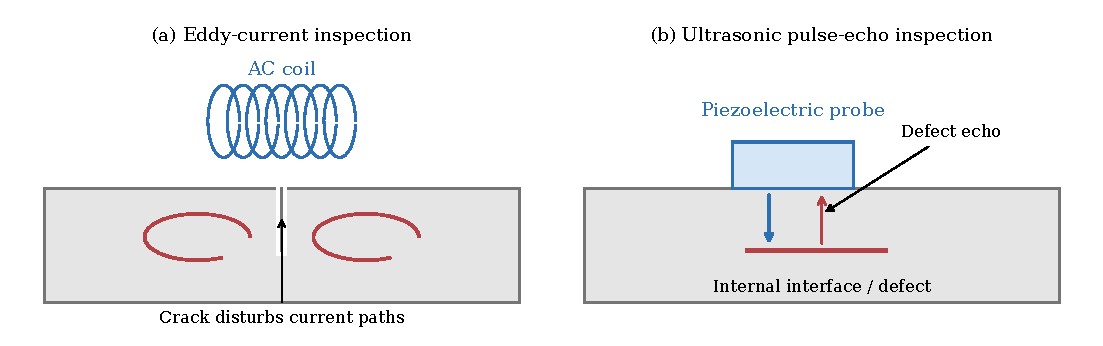
\includegraphics[width=.94\linewidth]{ch4-crack-detection.pdf}
\end{center}
\noindent 上图对比涡流受裂纹扰动和超声遇缺陷反射的机制；实际声束和扫描方向需依据叶片形状与预期裂纹取向设置。

\textbf{方法三：渗透显示配合光学检测。}对致密非多孔材料的\textbf{表面开口裂纹}，渗透液借毛细作用进入裂纹，去除表面多余渗透液后，经显像或荧光照明增强对比，再由相机等光电元件采集。它不能检出完全封闭在内部的裂纹，表面需清洁且开口不能被涂层遮挡。

\textbf{有条件的补充：磁性检测。}若叶片为\textbf{铁磁性材料}，磁化后裂纹附近会形成漏磁场，可由磁粉聚集显示，或由霍尔、磁阻等元件检测。该法不能因叶片“是金属”便直接采用，须先确认其磁性及磁化方向。

\subsection*{本题知识点与公式}\label{kn:4-5}
\noindent\textbf{已学前置：}\hyperref[kn:4-2]{第2题}已讲线圈、互感与涡流阻抗读出，\hyperref[kn:4-3]{第3题}已讲光电成像，\hyperref[kn:4-4]{第4题}已讲磁敏元件。本题新增无损检测的缺陷作用机制、趋肤深度和声学界面关系，重点是方法对材料、位置与取向是否成立。

\subsubsection*{1. 涡流为何改变探头阻抗}
涡流探头与导体可近似理解为一次线圈和一个分布式短路二次回路。用等效二次阻抗 $Z_s=R_s+\iu\omega_e L_s$、互感 $M$ 表示，二次感应电流为 $I_s=-\iu\omega_e MI_p/Z_s$，故一次端的反映阻抗为
\[
Z_{\mathrm{in}}=R_p+\iu\omega_e L_p+
\frac{\omega_e^2M^2}{R_s+\iu\omega_e L_s}.
\]
最后一项的实部代表附加损耗、虚部改变等效电感；这解释了为何实际检测通常同时分析阻抗幅值与相位。裂纹使局部电流绕行，改变等效耦合与阻抗，但抬离、边缘、曲率、涂层和材料变化也会改变这些量，因此异常信号需与参考试样及扫描位置对照。

\subsubsection*{2. 趋肤深度的来源、单位与频率选择}
均匀、线性、足够厚的良导体中，取时间因子 $e^{\iu\omega_et}$ 并忽略位移电流，麦克斯韦方程可化为一维磁场扩散方程
\[
\frac{\diff^2 H}{\diff z^2}=\iu\omega_e\mu\sigma_e H.
\]
沿深度 $z$ 衰减的解为
\[
H(z)=H(0)e^{-(1+\iu)z/\delta_s},\qquad
\boxed{\delta_s=\sqrt{\frac{2}{\omega_e\mu\sigma_e}}
=\sqrt{\frac{2\rho}{\omega_e\mu}}}.
\]
$\rho$ 是电阻率（$\Omega\,\mathrm m$），$\sigma_e=1/\rho$ 为电导率（S/m），$\mu$ 为绝对磁导率（H/m），$\omega_e=2\pi f_e$。把相对磁导率 $\mu_r$ 代入前须乘 $\mu_0$。$\delta_s$ 是场或电流密度幅值降至表面 $e^{-1}\approx36.8\%$ 的深度，既不是幅值降为零的位置，也不是通用的最大可检裂纹深度；相位还随深度滞后 $z/\delta_s$。

由 $\delta_s\propto f_e^{-1/2}\mu^{-1/2}\sigma_e^{-1/2}$ 可知，提高频率、磁导率或电导率都会减小标准穿透深度。高频有利于表层分辨，却更难深入；降低频率增加穿透，也可能降低细小表面缺陷的对比度。真实叶片的有限厚度、探头尺寸及弯曲表面不完全满足半空间模型，应把公式用于理解趋势与初选频率，再用试块验证。\footnote{趋肤深度及其幅值定义见\href{https://www.twi-global.com/technical-knowledge/faqs/faq-how-far-can-eddy-currents-penetrate}{TWI：How far can eddy currents penetrate?}；公式的均匀导体模型亦见\href{https://ansyshelp.ansys.com/public/views/secured/electronics/v242/en/subsystems/maxwell/content/SkinDepthforanEddyCurrentSolution.htm}{Ansys：Skin Depth for an Eddy Current Solution}。}

裂纹若大致平行于主涡流方向，阻断作用可能较弱；近似垂直于主电流路径时扰动更明显。故应改变扫描与励磁方向，而非只在某一位置读一次阻抗。涡流法要求导电，但并不要求铁磁；对铁磁材料，还需注意磁导率变化本身可能形成较强干扰。

\subsubsection*{3. 压电超声的发射、接收与缺陷回波}
压电材料的\textbf{正效应}把机械应力转为极化电荷，给定结构下可写 $Q=d_FF$，$d_F$ 单位为C/N；\textbf{逆效应}把电场转为机械应变，线性近似 $S=d_pE_e$，$d_p$ 单位为m/V，方向与晶体或陶瓷极化有关。探头发射利用逆效应，接收利用正效应；这两个过程组成“电信号 $\to$ 声波 $\to$ 缺陷反射 $\to$ 电信号”的完整链。

对均匀介质中的一维行波，特性声阻抗为
\[
Z_a=\rho_m c_s\quad
\bigl[\mathrm{kg/(m^2\,s)}\bigr],
\]
其中 $\rho_m$ 为质量密度，须与前面的电阻率 $\rho$ 区分。正常入射、平面界面、无损模型下，声压反射系数与强度反射率分别为
\[
r_p=\frac{Z_{a2}-Z_{a1}}{Z_{a2}+Z_{a1}},\qquad
\mathcal R_I=|r_p|^2.
\]
空气裂隙与金属的声阻抗差通常很大，能产生强反射；但探头与叶片之间若存在空气，也会阻碍声能进入工件，所以常需耦合剂或适当的非接触超声方案。式中 $r_p$ 可正可负，表示声压相位关系；$\mathcal R_I$ 是能量比，不能直接把两者相等。\footnote{声阻抗与界面反射的器件解释见\href{https://www.murata.com/products/sensor/ultrasonic/overview/basic/nature}{Murata：Properties of sound waves}；正常入射的反射关系可参见\href{https://hyperphysics.phy-astr.gsu.edu/hbase/Sound/acousimp.html}{Georgia State University：Acoustic Impedance}。}

在扣除仪器、耦合层及楔块延迟后，往返时间给出声程 $l=c_s\Delta t/2$。只有正入射且声程沿深度时才直接有 $h=l$；若声束在工件内与深度方向成角 $\theta$，则简单平面几何下 $h=l\cos\theta$。纵波、横波的声速不同，必须采用实际波型的材料声速。

探测能力还取决于波长 $\lambda_s=c_s/f_u$、脉冲长度、声束宽度与衰减。短脉冲有利于分开相邻回波，轴向分辨距离量级为 $c_s\tau_p/2$；提高频率通常改善小尺度分辨，却增加许多材料中的传播衰减。平面裂纹具有方向性，若镜面反射不返回接收探头，裂纹存在也可能回波弱，应采用多角度或阵列扫描。超声可用于适当声学条件下的金属、陶瓷等，不以导电或铁磁性为必要条件，但粗晶、薄壁和复杂曲面可能明显限制效果。

\subsubsection*{4. 磁性与渗透法各补充哪类缺陷}
磁粉与漏磁检测先磁化\textbf{铁磁性}工件。裂纹使磁路磁阻增大，局部磁通逸出表面；磁粉在漏磁场附近聚集，或由\hyperref[kn:4-4]{霍尔等磁敏元件}检测。缺陷对磁通的阻断程度随方向而变，必要时用两个励磁方向；非铁磁金属不能因为“导电”就直接采用磁粉法。

渗透法依靠润湿和毛细作用把液体带入\textbf{表面开口}裂纹，清除表面多余渗透液后显像，再作可见光或荧光观察。它对导电性、磁性没有上述要求，适用于合适的致密非多孔材料；封闭内部裂纹、被涂层堵住的开口和多孔表面都不宜直接套用。\footnote{原理及适用边界见\href{https://www-pub.iaea.org/MTCD/Publications/PDF/TCS-11.pdf}{IAEA：Liquid Penetrant and Magnetic Particle Testing}。}
因此本题若只要求“是否存在裂纹”，也应先规定材料和缺陷范围，再用相应参考缺陷建立判据；检测、定位和定量尺寸评估是不同层次的结论。
\nt{\textbf{易错点：}涡流需导电，磁性方法还需材料具有适用的磁性；两者不能混为一谈。超声发射用逆压电效应，接收用正压电效应，传播速度应取叶片材料内相应波型的声速。发现异常不等于已定量测出裂纹深度。}

\Needspace{11\baselineskip}
\section{第6题：光纤测压力与位移的工作原理}
\label{hw:4-6}
\begin{hwquestion}
说明用光纤传感器测量压力和位移的工作原理，指出其不同点。
\end{hwquestion}

\subsection*{答案与解析}
光纤可传输光，也可作为敏感元件。被测量改变光的强度、相位、偏振或波长，再由光电器件及解调电路读出。以\textbf{反射强度式光纤结构}说明两种测量，可直接比较其共同点与不同点。

\textbf{测位移：}发射光纤把光照向随被测对象移动的反射面，接收光纤收集反射光。间距 $d$ 改变时，光斑和接收耦合效率 $\eta(d)$ 改变，接收功率为
\[
P_r=P_t\eta(d),\qquad d=d_0+x.
\]
光电读出经标定后可将输出换为位移 $x$。应在 $\eta(d)$ 的合适单调区工作，避免同一输出对应两个间距。

\textbf{测压力：}把反射面制成受压弹性膜片。压力差 $p$ 使膜片产生位移 $x_d$，再改变光纤端面与膜片间距，从而改变接收光强。局部线性范围内可写
\[
p\longrightarrow x_d=k_pp
\longrightarrow d=d_0-x_d
\longrightarrow P_r=P_t\eta(d)\longrightarrow U_o.
\]
若光电及电路增益为 $G$，即 $U_o=GP_r$，则局部压力灵敏度为
\[
\frac{\diff U_o}{\diff p}=-GP_t\eta'(d)k_p.
\]
该式同时反映膜片机械灵敏度、光学耦合斜率和电路增益；输出正负取决于间距定义与工作分支。

\begin{center}
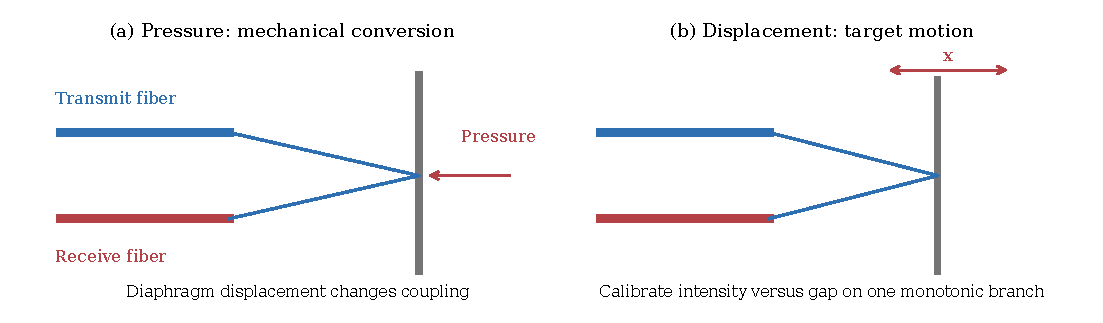
\includegraphics[width=.94\linewidth]{ch4-fiber-pressure-displacement.pdf}
\end{center}

\begin{center}
\small
\begin{tabularx}{\linewidth}{@{}p{2.1cm} X X@{}}
\toprule
比较项 & 位移测量 & 压力测量 \\
\midrule
机械输入 & 目标位移直接改变光学间距。 & 压力先使膜片等弹性体变形，再改变光学间距或应变。 \\
共同读出 & \multicolumn{2}{p{11.5cm}@{}}{均可采用强度、相位或波长调制；上述示例均用反射强度调制和光电转换。} \\
主要标定 & 光路、反射率、间距与输出关系及单调工作区。 & 除光学读出外，还需标定膜片刚度、温度及压力差边界条件。 \\
动态限制 & 目标运动与光电读出带宽。 & 还受膜片固有频率、阻尼及压力传递过程限制。 \\
\bottomrule
\end{tabularx}
\end{center}

\subsection*{本题知识点与公式}\label{kn:4-6}
\noindent\textbf{已学前置：}光到电的响应度和读出见\hyperref[kn:4-3]{第3题}，机械应变见\hyperref[kn:4-1]{第1题}，机械幅相响应见\hyperref[kn:3-3]{二阶系统知识点}。本题新增导光条件、三类光学调制和压力到光学量的弹性转换，重点解释压力与位移测量为何可共用同一光学读出。

\subsubsection*{1. 光纤如何导光，为什么间距会改变接收光}
普通阶跃型光纤由折射率较高的纤芯 $n_1$ 和较低的包层 $n_2$ 构成，$n_1>n_2$。在几何光学的子午光线近似下，纤芯到包层的入射角相对法线大于临界角
\[
\theta_c=\arcsin(n_2/n_1)
\]
时发生全反射。若外部介质折射率为 $n_0$，入射光相对纤轴的最大接收半角为 $\theta_a$，由端面折射和全反射条件可得数值孔径
\[
\boxed{\mathrm{NA}=n_0\sin\theta_a=\sqrt{n_1^2-n_2^2}}.
\]
数值孔径无量纲，描述可接收光锥的范围；不是越大测量就必然越准。上述光线公式适用于相应阶跃型导光模型，单模光纤的场分布和耦合还需波动光学描述。\footnote{全反射和接收角关系见\href{https://bop-iitk.vlabs.ac.in/exp/numerical-aperture-measurement/theory.html}{IIT Kanpur Virtual Labs：Numerical aperture measurement}。}

反射强度式探头的发射光形成扩展光斑，反射后只有落入接收纤端面且角度满足耦合条件的部分进入光纤，所以 $P_r=P_t\eta(d)$ 随间距改变。这里 $\eta$ 是包括光路几何与反射损失的耦合效率，不是第3题的量子效率 $\eta_q$。$\eta(d)$ 往往有峰值和不同斜率分支，需选定单调区；小变化时 $\Delta P_r\approx P_t\eta'(d_0)\Delta d$，在峰值处 $\eta'\approx0$，反而不适合灵敏位移读出。参考光路或比值 $P_r/P_{\mathrm{ref}}$ 可减轻共同光源功率波动，但不能自动消除目标反射率、弯曲损耗与几何变化。

\subsubsection*{2. 压力多了一段弹性机械转换}
位移测量中，目标运动直接使间距变化。压力是单位面积上的法向载荷（Pa），反射膜片受到的通常是两侧\textbf{压力差} $p=p_{\mathrm{in}}-p_{\mathrm{out}}$，并非没有参考条件的绝对压力。

以半径 $a$、厚度 $t_m$、周边固支的均匀圆形薄膜片为明确模型。材料各向同性、线弹性，均匀压力下的小挠度板弯曲刚度为
\[
D_b=\frac{Et_m^3}{12(1-\nu^2)}.
\]
$D_b$ 单位为N$\cdot$m。薄板方程 $D_b\nabla^4w=p$ 配合边缘条件 $w(a)=0$、$w'(a)=0$，得到
\[
w(r)=\frac{p}{64D_b}(a^2-r^2)^2,
\qquad
\boxed{w_0=\frac{pa^4}{64D_b}
=\frac{3(1-\nu^2)pa^4}{16Et_m^3}}.
\]
这里 $w_0$ 为中心挠度，$E$ 的单位为Pa，$a,t_m,w_0$ 均用m；模型要求薄板、挠度相对厚度足够小、无显著初始张力及塑性，边界确为固支。大挠度时膜内拉力变得重要，不能继续把上式线性外推。其他膜片形状、波纹和支承方式的系数也不同。\footnote{固支圆板的边界条件与解见\href{https://pkel015.connect.amazon.auckland.ac.nz/SolidMechanicsBooks/Part_II/06_PlateTheory/06_PlateTheory_05_RectangularCoordinates.pdf}{P. Kelly：Solid Mechanics Part II，Section 6.5}。}

于是本题示例的 $k_p=w_0/p$ 单位为m/Pa。若间距 $d=d_0-w_0$、光电总增益 $G$ 的单位为V/W，便有
\[
\frac{\diff U_o}{\diff p}=
\underbrace{G}_{\text{电路与光电}}
\underbrace{P_t\eta'(d)}_{\text{光学耦合}}
\underbrace{(-k_p)}_{\text{压力到位移}},
\]
输出灵敏度单位为V/Pa。增大半径或减薄膜片会提高静态灵敏度，也会降低刚度并影响固有频率、过载与线性范围。把膜片的主模态近似为二阶系统时，其归一化幅相规律沿用\hyperref[kn:3-3]{测试系统的二阶模型}；测压系统还可能受到引压管、腔体及光电读出带宽限制。

\subsubsection*{3. 相位式：读光程，不只读光强大小}
两束相干光叠加时，探测强度可写
\[
I=I_1+I_2+2V_c\sqrt{I_1I_2}\cos\Delta\phi,
\quad 0\le V_c\le1.
\]
$V_c$ 是可见度相关因子，反映相干、偏振和空间重叠等条件。反射腔的往返相位含 $\Delta\phi=4\pi nd/\lambda+\phi_0$；当折射率 $n$ 固定时，$\Delta(\Delta\phi)=4\pi n\Delta d/\lambda$。单个强度读数对相位是周期且多值的，小位移常在正交工作点附近线性读出，大范围位移则需条纹计数或相位解缠；一整条纹对应间距变化 $\lambda/(2n)$。温度也能改变 $n$、腔长和参考光程，需稳定或补偿。

压力若通过膜片改变同一腔长，也能用上述相位式读出；因此“位移只能调强度、压力只能调相位”没有普遍依据。

\subsubsection*{4. FBG波长式与温度补偿}
FBG是在纤芯中形成的周期性折射率调制结构。相邻周期的反射光满足相干增强条件 $2n_{\mathrm{eff}}\Lambda=\lambda_B$，所以反射中心波长为
\[
\lambda_B=2n_{\mathrm{eff}}\Lambda,\qquad
\frac{\Delta\lambda_B}{\lambda_B}
\approx\frac{\Delta n_{\mathrm{eff}}}{n_{\mathrm{eff}}}
+\frac{\Delta\Lambda}{\Lambda}.
\]
轴向应变既改变光栅周期，也通过弹光效应改变有效折射率；温度通过热膨胀和热光效应改变两者。对相应自由光纤、小变化模型，可写
\[
\boxed{\frac{\Delta\lambda_B}{\lambda_B}
=(1-p_e)\varepsilon+(\alpha_f+\xi)\Delta T},\qquad
\xi=\frac{1}{n_{\mathrm{eff}}}\frac{\partial n_{\mathrm{eff}}}{\partial T}.
\]
$p_e$ 为有效弹光系数，$\alpha_f,\xi$ 单位为$\mathrm K^{-1}$；这里 $\varepsilon$ 表示额外机械应变，热膨胀另列。粘贴和封装会改变应变传递及温度系数，工程上应采用标定后的 $K_\varepsilon,K_T$，写成相对波长变化 $K_\varepsilon\varepsilon+K_T\Delta T$。若压力经弹性结构产生 $\varepsilon=k_{\varepsilon p}p$，即可得到压力读出，但不能从一个未知温度下的波长漂移唯一分离应变与温度。\footnote{FBG机械与温度响应及封装影响见\href{https://www.hbm.com/fileadmin/mediapool/files/technical-articles-technotes-white-papers/Article_Sensing_of_Surface_Strain_with_Flexible_Fiber_Bragg_Strain_Gages_2011_EN.pdf}{HBM：Sensing of Surface Strain with Flexible Fiber Bragg Strain Gages}。}

温度补偿可增加一个同温、机械隔离的参考光栅，先由其波长求 $\Delta T$ 再扣除温度项；或使用两个灵敏度不同、方程相互独立的光栅联合求解。对粘贴在构件上的光栅，还应区分构件真实热变形与光栅自身的温度交叉影响。光纤抗电磁干扰是传输与光学敏感段的优点，光源、探测器和解调仪仍需供电、标定与带宽核查。
\nt{\textbf{易错点：}光纤抗电磁干扰并不意味着整个系统没有漂移。强度式结构受光源功率、弯曲损耗、反射率等影响；压力式还受弹性体温度、迟滞和机械动态影响。光纤传感器也并非全部非接触。}

\needspace{11\baselineskip}
\section{第7题：传感器选用的基本原则}
\label{hw:4-7}
\begin{hwquestion}
选用传感器的基本原则是什么？
\end{hwquestion}

\subsection*{答案与解析}
原则是\textbf{从实际测量任务出发，在满足测量要求的前提下，综合比较可靠性、可实现性和总成本}。不能仅凭灵敏度或标称精度最高作选择，可按以下顺序筛选。

\begin{enumerate}
\item \textbf{明确被测对象与可测性。}规定被测量、量程、最大过载、最小有意义变化、静态或动态特征、接触条件与安装空间。先判断机理是否适用，例如涡流需导电对象；长期静态力不宜直接依赖存在电荷泄漏的压电读出。
\item \textbf{确定准确度与分辨力要求。}综合非线性、迟滞、重复性、零漂、温漂、交叉敏感和噪声，评估整个测量链的误差，而非只看敏感元件的某一个指标。量程应覆盖最大输入并留有适当裕量，同时避免量程过大导致小信号难辨。
\item \textbf{核查动态性能。}在关注频带内，幅值误差和相位误差应满足要求，并考虑响应时间、固有频率、阻尼及安装后的整体结构。元件本身响应快，不保证装配后的测量系统有同样带宽。
\item \textbf{选择合适灵敏度与输出形式。}小信号应能高于噪声和分辨阈值，最大信号又不能使后级饱和；核查激励、输出阻抗、放大、解调、滤波、采样和接口是否匹配。
\item \textbf{适应现场环境并减小测量扰动。}考虑温湿度、腐蚀、振动冲击、粉尘、防护和电磁环境；同时检查接触力、刚度、质量加载、自热等是否改变被测对象。
\item \textbf{保证可安装、可校准、可维护。}比较尺寸、接线、校准条件、长期稳定性、互换性、寿命、供货与维护成本。在性能足够时，优先选择结构可靠、已有使用经验且便于标定的方案。
\end{enumerate}

\subsection*{本题知识点与公式}\label{kn:4-7}
\noindent\textbf{已学前置：}前6题给出各敏感机理及适用材料，\hyperref[kn:3-1]{测试系统知识点}已讲频响。本题新增静态性能指标的严格含义、误差归一化和完整测量链匹配，用统一量纲把这些方案放在同一任务中比较。

\subsubsection*{1. 先规定测量范围、参考关系与误差分母}
设输入 $x\in[x_{\min},x_{\max}]$，输入量程跨度 $X_{\mathrm{FS}}=x_{\max}-x_{\min}$，标定输出为 $y$，参考直线为 $y_{\mathrm{ref}}=b+S_0x$，其输出跨度为 $Y_{\mathrm{FS}}=|S_0|X_{\mathrm{FS}}$。\textbf{测量范围}描述上下限，\textbf{量程跨度}描述两者之差；双极性范围不能把正端上限当成整个跨度。过载能力说明超出正常范围后的承受能力，不保证在过载区仍符合原准确度。

输入估计值 $\hat x$ 的绝对误差为 $e_x=\hat x-x_{\mathrm{ref}}$，单位与输入相同。相对误差 $e_x/x_{\mathrm{ref}}$、读数百分比和满量程百分比 $100e_x/X_{\mathrm{FS}}$ 使用不同分母，不能只写“误差1\%”而不说明基准。输入接近零时，按读数定义的相对误差可能很大或无定义，此时应给绝对误差、零点误差或按跨度归一化的指标。

\subsubsection*{2. 灵敏度、分辨力与准确度不能互相代替}
\textbf{灵敏度}是输入变化引起的输出变化率：
\[
S(x_0)=\left.\frac{\diff y}{\diff x}\right|_{x_0},\qquad
\Delta y\approx S(x_0)\Delta x.
\]
单位为“输出单位/输入单位”，例如V/Pa。线性标定中 $S_0$ 为常数，非线性传感器则需指定工作点。相对灵敏度 $(\diff y/y)/(\diff x/x)=Sx/y$ 无量纲，但要求所用 $x,y$ 不为零且参考定义明确。\textbf{分辨力}是在给定噪声、观察时间和判别规则下能区分的最小输入变化，局部可估为 $\Delta x_{\min}\approx\Delta y_{\min}/|S|$；第1题正是缺少 $\Delta y_{\min}$，不能仅凭输出变化就确定可读性。

\textbf{准确度}描述测量结果与真值或认可参考值的接近程度，受系统偏差和随机变化共同影响；\textbf{精密性}描述规定条件下重复结果的接近程度。日常“精度”可能指两者中的不同含义，答题时应给实际误差限或重复性指标。灵敏度高但温漂、迟滞大，准确度仍可能较差；数字位数多也不能消除系统偏差。

\subsubsection*{3. 线性度、迟滞与重复性分别怎样量化}
\textbf{非线性误差}是实际标定曲线相对选定参考直线的最大偏差。常见输出跨度归一化定义为
\[
\delta_L=\frac{\max_x|y(x)-y_{\mathrm{ref}}(x)|}{Y_{\mathrm{FS}}}\times100\%.
\]
端点直线、最小二乘直线和其他最佳拟合直线会给出不同结果，须说明参考方法，不能混用分子和分母。非线性可通过标定补偿，但补偿后的误差还受温度、噪声及模型稳定性限制。

\textbf{迟滞}是在同一输入、相同环境下，增程与减程输出不同，常定义
\[
\delta_H=\frac{\max_x|y_{\uparrow}(x)-y_{\downarrow}(x)|}
{Y_{\mathrm{FS}}}\times100\%.
\]
它与只沿一个方向测量得到的非线性不同，常与摩擦、磁滞或材料内部过程有关。\textbf{重复性}是在相同程序、同方向、短时间及相同条件下重复施加同一输入，输出的离散程度。对 $m$ 次读数可计算
\[
\bar y=\frac1m\sum_{i=1}^{m}y_i,\qquad
s_y=\sqrt{\frac{\sum_{i=1}^{m}(y_i-\bar y)^2}{m-1}}.
\]
若用极差、$s_y$ 或 $ks_y/Y_{\mathrm{FS}}$ 作为重复性指标，应明确统计量、$k$、次数及是否归一化。重复性好不能证明无固定偏差；不同设备、操作者或长期条件下的再现性也不等于同条件重复性。

\subsubsection*{4. 零漂、灵敏度漂移与交叉敏感}
在输入不变时，输出随时间或环境变化称漂移。\textbf{零点漂移}改变截距，\textbf{灵敏度漂移}改变斜率。在温度小范围内，可表示为
\[
y\approx b_0+S_0x+k_{0T}\Delta T+S_0\alpha_Sx\Delta T.
\]
$k_{0T}$ 是输出零点温度系数（如V/K），$\alpha_S$ 是相对灵敏度温度系数（$\mathrm K^{-1}$）。零漂也可折算到输入为 $k_{0T}/S_0$（如Pa/K），或再除以跨度表示\%FS/K；不同表示不能仅比数字大小。长期漂移需给时间尺度，不能用短时重复测量替代。

更一般地，非目标量 $z$ 也改变输出，局部模型为
\[
\Delta y\approx S_x\Delta x+S_z\Delta z,
\qquad \Delta x_{\mathrm{eq}}=\frac{S_z}{S_x}\Delta z.
\]
$S_z$ 为交叉灵敏度，$\Delta x_{\mathrm{eq}}$ 是其等效输入误差。应变片的温度、反射式传感器的表面反射率、FBG的温度都是本章已出现的实例。只有温度项和载荷项得到独立信息或合理补偿，才可把输出归因于目标输入。

\subsubsection*{5. 噪声、动态与接口如何形成系统限制}
若多个线性环节的局部增益为 $S_1,S_2,\ldots,S_n$，总灵敏度为 $S_{\mathrm{tot}}=\prod S_i$。输出端噪声均方根为 $\sigma_y$ 时，等效输入噪声近似为 $\sigma_x=\sigma_y/|S_{\mathrm{tot}}|$；若规定需超过噪声若干倍才能判别，应明确该倍数及统计假设，不能把一个标准差自动当成确定的最小可测量。

量化也产生限制：若ADC满量程电压跨度为 $V_{\mathrm{span}}$、有效采用 $n_b$ 位均匀码级，则理想码宽 $q_v\approx V_{\mathrm{span}}/2^{n_b}$，可折算成 $q_x=q_v/|S_{\mathrm{tot}}|$。实际有效位数、噪声与漂移可能比理想码宽更差。放大应使最小信号可辨，同时确保最大正常信号、零偏及暂态不会使后级饱和。

\textbf{带宽}必须按幅相允许误差或指定截止定义。$-3\,\mathrm{dB}$ 处的幅值已降至约 $0.707$，不等于高精度测量仍无失真。各环节频响相乘 $H_{\mathrm{tot}}(\iu\omega)=\prod H_i(\iu\omega)$，幅值比相乘、相位相加；实际可用测量频带需满足整体误差目标，推导沿用\hyperref[kn:3-1]{第3章一阶响应}和\hyperref[kn:3-3]{二阶响应}。冲击过载还需检查是否激起结构共振。

\textbf{加载效应：}电压输出的戴维南源阻抗为 $Z_s$、后级输入阻抗为 $Z_{\mathrm{in}}$ 时，$U_{\mathrm{read}}=U_{\mathrm{oc}}Z_{\mathrm{in}}/(Z_s+Z_{\mathrm{in}})$。减轻电压加载通常要求工作频带内 $|Z_{\mathrm{in}}|\gg|Z_s|$，并核查相位。机械接触、附加质量与刚度也会改变对象运动，须在实际安装状态下检查。

选型时先规定量程、最小变化、频带、材料和环境，再按同一输入单位、明确误差分母比较整条链的噪声、漂移与误差。没有这些任务指标，不能只凭原理名称确定唯一最优型号。
\nt{\textbf{易错点：}灵敏度、分辨力、准确度、稳定性与带宽须分别核查；单项指标高不代表整条测量链满足任务。}
